\documentclass{article}
\usepackage{graphicx}
\begin{document}
\oddsidemargin0cm
\topmargin-2cm
\textwidth16.5cm
\textheight23.5cm
\begin{quote}
\begin{verbatim}
                                  BYLAWS
                                   KGB

                                ARTICLE I
                           NAME AND OBJECTIVES

Section 1. The name of the organization shall be KGB.

Section 2. The objectives of the organization shall be:

    a. to promote a spirit of fellowship among its members.

    b. to take an active and positive role in campus life.

Section 3. The organization shall not be conducted or operated for
profit and no part of any profits or remainder or residue from dues,
donations, or other sources of income to the organization shall inure
to the personal benefit of any member or individual.

                               ARTICLE II
                               DEFINITIONS

Section 1. Standing Definitions. The terms defined as follows shall be
considered standing definitions:

    a. Majority. A majority shall be defined as a number greater then
    one-half (1/2), or fifty percent (50%), of the total.

    b. Organization Quorum. A quorum of the organization is required in
    order to hold meetings as set forth in Article IV, Sections 1 and 2,
    and shall be either a majority of the voting members or seventy-five
    percent (75%) of the active members.

    c. Board Quorum. A quorum of the Board is required in order to hold
    meetings set forth in Article IV, Sections 3, 4, and 5, shall be a
    majority of the Board members.

    d. Written Petitions. All written petitions shall bear the signatures
    of either ten (10) members, or twenty percent (20%) of the voting
    membership, whichever is greater.

    e. Member in Good Standing.  A member is in good standing whose dues
    are current and whose other monetary obligations to the organization
    are fulfilled
         1) within sixty (60) days of the obligation's creation, or 2)
         by the Annual Meeting (as defined in Art. VI, Sec. 2)
    whichever comes first unless such obligations are created within
    seven (7) days prior to the Annual Meeting, in which case clause 2
    shall not apply.

    f. Voting Member. A voting member is a member in good standing who
    has attended at least one (1) previous meeting during their current
    term of membership.

    g. Mailing. A mailing may be by physical or electronic means.
    Such mail must be individually addressed to each recipient, and may
    not only be to a single central bulletin board or other medium.

    h. Active Member.  An active member shall be a voting member who has
    attended at least one of the three (3) previous regular organization
    meetings as set forth in Article IV, Section 1 of these bylaws.

    i. Annual Meeting.  The annual meeting is the meeting at which the
    officers shall be elected for the ensuing year, and at which other
    significant business is conducted in accordance with these bylaws,
    and is described in Article VI, Section 2 of these bylaws.

    j. Random Process.  A random process shall be any method of choice
    which assigns an equal probability of selection to each option.

    k. Duck. Anything that looks like a duck, walks like a duck, and
    quacks like a duck.

    l. Zombie Dollar.  One zombie dollar is the equivalent of the fee
    assessed members with a body temperature equal to or less than
    fifty (50) degrees Fahrenheit, as defined in Article III, Section
    2 of these bylaws.

    m. Term of Membership.  A member's term of membership is the length
    of time covered by their most recent payment of dues, or the period
    dating back to when they most recently became a member of KGB, 
    whichever is shorter.

Section 2. Provisional Definitions. All terms not previously defined as
standing Definitions shall be defined according to the current edition
of MERRIAM-WEBSTER'S COLLEGIATE DICTIONARY.

                               ARTICLE III
                               MEMBERSHIP

Section 1. Membership. Each individual voting member shall have one (1)
vote. Each member shall receive one (1) copy of any notices, publications
or other distributed documents of the organization.

Section 2. Becoming a Member.  Any person whose dues have been paid to
the Treasurer and whose body temperature is above fifty (50) degrees
Fahrenheit shall be considered a member.  However, the second requirement
can be waived for the fee of siz (6) dollars. The KGB abides by the
Carnegie Mellon Statemen tof Assurance.

Section 3. Dues. Membership dues for the next year shall be suggested
annually by the Executive Board in March, and approved or changed by
the voting membership at the April meeting.  Dues shall be payable on
or before the thirtieth day of September each year.

Section 4. Termination. Memberships may be terminated voluntarily:

    a. by resignation. Any member may resign from the organization upon
    written notice to the Recording Secretary.

    b. by lapsing. A membership will be considered as lapsed and
    automatically terminated if such member's dues remain unpaid thirty
    (30) days after the deadline for payment of dues.  However, the
    Executive Board may grant an additional thirty (30) days grace period
    to such delinquent members in exceptional cases. In no case may a
    person be entitled to vote at any organization meeting whose dues
    are unpaid as of the date of that meeting, or who are sixty (60)
    days in arrears of other monetary obligations to the organization.

Section 5. Refund of Dues. Membership dues will not be refunded either
wholly or in part for any reason save extreme circumstances as determined
by the membership.

Section 6. Benefits of Membership. All members in good standing shall
receive all benefits of membership except as stipulated in the bylaws.


                               ARTICLE IV
                           MEETINGS AND VOTING

Section 1. Regular Organization Meetings. Regular meetings of the
organization shall be held as directed by the Executive Board.  Written
notice of such meetings shall be mailed to the membership at least six
(6) days prior to the date of the first such meeting of each semester by
the Corresponding Secretary through the official organization newsletter
or by other mailing, as well as upon any change in the announced time.

Section 2. Special Organization Meetings. Special meetings of the
organization may be called by the President, or by a majority vote of
the members of the Executive Board who are present and voting at any
regular or special meeting of the Board, or by the Recording Secretary
upon receipt of a written petition.  Written notice of such meetings shall
be mailed by the Corresponding Secretary at least three (3) and not more
than fifteen (15) days prior to the date of the meeting. Such notice
shall state the purpose(s) of the meeting, and no other organization
business may be transacted thereat.

Section 3. Regular Executive Board Meetings. Regular meetings of the
Executive Board shall be held as directed by the Board, with a minimum
of two (2) such meetings per semester.  Notice of such meetings shall
be mailed to the membership at least six (6) days prior to the date of
the first such meeting of each semester by the Corresponding Secretary
and upon any change in the announced time.  Such meetings shall be
closed to non-members of the organization unless the individual(s)
should be specifically invited by the Board, in which case the cause
for the non-member presence shall be the first order of business, and
after which the non-member may be asked to leave the meeting.

Section 4. Special Executive Board Meetings. Special meetings of the
Executive Board may be called by the President, or by the Recording
Secretary upon the receipt of a written petition signed by at least three
(3) members of the Board.  Notice of such meetings shall be given to the
membership at least five (5) days prior to the meeting.  Such notice
shall state the purpose of the meeting and no other business may be
transacted thereat.  In addition, all restrictions in Section 3 of this
article shall apply to special meetings of the Board.

Section 5. Emergency Board Meetings.  Emergency meetings of the Board
may be called by the President or First Vice-President and may be held
by phone.  Notice of such meetings shall be given to the officers at
least one (1) day prior to the meeting.  Any majority decision reached
will be entered into the minutes of the next regular Board meeting.

Section 6. Voting. Each voting member shall be entitled to one (1) vote at
any regular meeting of the organization at which the member is present.
Absentee voting will be permitted only for elections.  Absentee ballots
must be submitted to all the election proctors at least twelve (12)
hours in advance of the commencement of the Annual Meeting, unless the
proctors decide to accept absentee ballots after this deadline. Absentee
ballots may be submitted by electronic mail, in person, or by any other
method the proctors deem acceptable.

                                ARTICLE V
                      OFFICERS AND REPRESENTATIVES

Section 1. Executive Board. The officers of the organization shall
constitute the Executive board.  The power necessary for the general
management of the organization's affairs shall be entrusted to the Board,
except as follows.

    a. The Board shall be subject to the orders of the organization, and
    none of its acts shall conflict with action taken by the organization,
    and the organization may countermand any decision of the board by
    a majority vote, thus opening up the question for consideration by
    the organization.

    b. The Board shall not distribute the organization's funds except
    as directed by the organization.

Section 2. Officers. The organization officers, consisting of the
following, shall serve in their respective capacities both with regard
to the organization and its meetings and the Board and its meetings.

    a. The President shall preside at all meetings of the organization
    and of the Board, and shall have the duties and powers normally
    applicable to the office of President in addition to those provided
    for in these bylaws.

    b. The First Vice-President shall be in charge of fellowship and
    shall actively recruit new members.

    c. The Second Vice-President shall be in charge of organizing
    fellowship activities.

    d. The Corresponding Secretary shall have charge of all correspondence
    pertinent to the organization other than the correspondence reserved
    for the Recording Secretary and Treasurer.  The Corresponding
    Secretary shall be the Editor of the organization Newsletter.

    e. The Recording Secretary shall keep a record of all meetings
    of the organization and of the Board and of all matters of which a
    record shall be ordered by the organization.  The Recording Secretary
    shall keep a roll of the members of the organization with applicable
    information, including attendance at meetings of the general body;
    furthermore, the Recording Secretary shall carry out such other
    duties as are prescribed in these bylaws, and shall have the duties
    and powers normally applicable to the office of Secretary, except for
    those duties and powers assigned to another officer by these bylaws.
    In the absence of the Recording Secretary, the duties and powers
    thereof shall be executed by the Corresponding Secretary, or in the
    absence thereof, the most senior officer present not presiding over
    the meeting.

    f. The Treasurer shall collect and receive all moneys due or
    belonging to the organization, and shall deposit the same in a
    bank satisfactory to the Board, in the name of the organization.
    The Treasurer's books shall be open at all times to the inspection of
    the Board, and the Treasurer shall report to the Board and the general
    membership at every meeting the condition of the organization's
    finances. At the annual meeting, the Treasurer shall render an
    account of all moneys received and expended during the previous
    fiscal year. During the month of September the Treasurer shall
    mail to each member a statement of dues for the ensuing year. The
    Treasurer shall disperse funds as directed by the Executive Board.
    The Treasurer shall also be responsible for filing all financial forms
    applicable to the organization.  In the absence of the Treasurer, the
    Recording Secretary shall record allocations made or debts incurred
    by or to the organization; however, the Recording Secretary shall not
    disburse or collect moneys, unless authorized so to do by the Board.

    g. The Sergeant-at-Arms shall assist in preserving order as the
    chair may direct, and other duties as set forth in the standing
    rules of order.

Section 3. Officer Requirements. All Officers of the organization shall
be voting members who are Activities Fee-paying students.

Section 4. Vacancies. Any vacancy of an officer position occurring on the
Board during the year shall be filled for the unexpired term of office by
a majority vote of all the remaining members of the Board by the second
regular meeting of the board following the creation of such vacancy.

Section 5. Recall of Officers. Any officer may be recalled for misconduct
or dereliction of duty. A written petition, stating the reason(s)
for recall, shall be filed with the Board.  Written notice of such a
petition shall be mailed to the membership.  At the next regular meeting
at least six (6) days after the mailing, a hearing on the matter will be
held and a two-thirds (2/3) vote will be required to sustain the recall.

Section 6. Seniority. Seniority of offices is: President, First
Vice-President, Second Vice-President, Corresponding Secretary, Recording
Secretary, Treasurer, and Sergeant-at-Arms.

                               ARTICLE VI
                           MUSICAL INTERLUDE
\end{verbatim}
\begin{center}
\scalebox{.75}{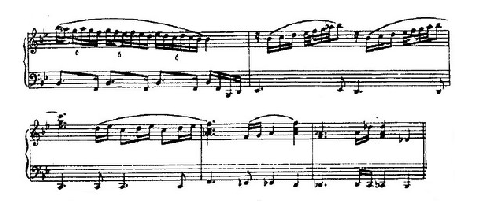
\includegraphics{MusicalInterlude.png}}
\end{center}

\begin{verbatim}

                               ARTICLE VII
              ORGANIZATION YEAR, ANNUAL MEETING, ELECTIONS

Section 1. Organization Year. The organization's fiscal year shall begin
on the first day of September and end on the thirty-first day of August.
The organization's official year shall begin immediately at the conclusion
of the election at the annual meeting and shall continue through the
election at the next annual meeting.

Section 2. Annual Meeting. No later than the last meeting in the
month of December the board shall set the date for the Annual Meeting.
The annual meeting shall be held in the month of April of each year.
At the Annual Meeting the Officers for the ensuing year shall be elected
by secret, written ballot from among those nominated in accordance with
Section 4 of this article. They shall take office immediately upon the
conclusion of the election and each retiring officer shall relinquish
all properties and records relating to that office within fifteen (15)
days after the election.

Section 3. Elections. The color of elections shall be purple.

    a. Proctors.  For the duration of the elections at the Annual Meeting,
    a set of at least three proctors shall preside and keep order at
    the meeting.  Ballots shall be counted by at least two proctors.
    Proctors shall be ineligible to run in that year's elections.
    Proctors shall be voting members of the organization except as
    discussed in section VI.3.b.

    b. Normal Proctor Selection.  At least two weeks prior to the
    Annual Meeting, a slate of at least three consenting members shall
    be nominated as proctors at a meeting of the Board.  A member
    shall not be nominated if any member of the Board objects.  At any
    meeting of the general body thereafter prior to the Annual Meeting,
    the slate may be modified or approved by a two-thirds (2/3) vote.
    At any such time, if it has not yet approved a slate of proctors,
    the organization may elect to request proctors from an external
    source with a two-thirds (2/3) vote.

    c. Emergency Proctor Selection.  If, at the Annual Meeting, less
    than three approved proctors are in attendance, the general body
    shall again have the opportunity to modify and approve the slate
    of proctors.  If no proctors have yet been approved, after at least
    two failed votes to approve the current slate of proctors the chair
    may declare an impasse.  In such an impasse, five present members
    not presently nominated for office shall be selected as proctors
    by random process; or, if five such members cannot be found, five
    members from the total attendance shall be so selected, but shall
    remain eligible for election.

    d. Election Procedure.  The election of each officer shall be
    concluded before the election of the next begins, and these elections
    shall be held in order of the chain of command. Write-in ballots
    or other invalid ballots shall be considered as abstentions. The
    candidate receiving a majority of the votes cast for each office shall
    be declared elected. In the case of an all-way tie, an additional
    round shall be run. Should the tie repeat, the winner shall be
    decided by the proctors of the election by random process. Otherwise,
    candidates shall be eliminated by the following method:

        1) Sort candidates into tiers of people with the same number
        of votes.

        2) Starting with the lowest ranking tier, remove tiers from the
        running in increasing order of rank until removing another would
        bring the total number of votes removed above 1/3. If there are
        no tiers with a number of votes below 1/3, remove the lowest
        ranking tier.

        3) If more than one candidate remains, run another round.

    The winner shall be announced by the election proctors. At least
    three of the election proctors shall sign a document in triplicate
    containing the names of the new executive board. Vote totals shall
    not be announced. The ballots shall be destroyed upon completion of
    the elections.

    e. Election Quorum.  Election of officers may proceed in the absence
    of quorum if the presence at the meeting of every absentee voter would
    be sufficient to reach quorum.


Section 4. Nominations. No person may be a candidate in an organization
election who has not been nominated or who is not a voting organization
member in good standing. During the last quarter of the official year the
Executive Board shall select a Nominating Committee consisting of four
(4) members willing to so serve, not more than one (1) of whom shall
be a member of the Board. The Recording Secretary shall immediately
notify the committee members of their selection.  The Board shall name a
Chairperson for the committee and it shall be this person's duty to call
a committee meeting which shall be  held on or before March 1. Once the
first meeting has been held, the membership of this committee cannot
be altered by the board. No person who has served on the Nominating
Committee will be eligible to run in that year's elections.

    a. The committee shall encourage as many able members to nominate
    themselves for offices as possible. If any office has no nominations
    for candidates, one (1) week before nominations are closed,
    Nominating Committee shall nominate one (1) person to that position,
    and after securing the consent of each person so nominated, shall on
    or before the fourth day before nominations are closed report their
    nominations to both the Recording and Corresponding Secretaries in
    writing. Nominating Committee is to do everything in its power to
    maintain the appearance of neutrality.

    b. Upon receipt of the Nominating Committee's report, the
    Corresponding Secretary shall on or before the third day before
    nominations are closed notify each member in writing of the candidates
    so nominated.

    c. Additional nominations may be made at any meeting after the report
    of the nominating committee and before the annual meeting by any
    member in attendance provided that the person so nominated does not
    decline when his or her name is proposed, and provided further that
    if the proposed candidate is not in attendance at this meeting,
    the proposer shall present to the Recording Secretary a written
    statement of the candidate's willingness to be so nominated.
    A voting member may be nominated and run for more than one (1)
    office, but shall only be allowed to hold one (1) office.

    d. Upon finalization of the nominations and at least three days
    before the annual meeting, the Corresponding Secretary shall notify
    each member in writing of the list of candidates.

    e. Nominations cannot be made at the annual meeting or in any manner
    other than as provided for in this section.

                               ARTICLE VIII
                                COMMITTEES

Section 1. The Board may each year appoint standing ordinary committees
to advance the work of the organization. Special ordinary committees may
also be appointed by the Board to aid it on particular projects. Such
committees shall always be subject to the final authority of the Board.

Section 2. Any ordinary committee appointment may be terminated by the
Board upon written notice to the appointee, and the Board may appoint
successors to those persons whose services have been terminated.

Section 3. The organization may appoint extraordinary committees to
advance the work of the organization.  Each such committee has an owner,
who must be a member in good standing of the organization.  The owner
appoints and replaces the chair of the committee as deemed appropriate.

Section 4. The owner of an extraordinary committee is determined
by auction, the proceeds of which are payable to the organization.
In the event of a vacancy in ownership of an extraordinary committee,
the organization may fill the vacancy by auction.

Section 5. The owner of an extraordinary committee may transfer the
ownership of the committee to another member in good standing by notifying
the Recording Secretary.

Section 6. The Recording Secretary shall maintain a record of the
membership of all ordinary committees and of the ownership of all
extraordinary committees.

                              ARTICLE IX
                  REPRIMAND, SUSPENSION, AND EXPULSION

Section 1. Any member of the organization shall be held accountable for
any conduct considered injurious to the organization or its purposes
and objectives. The gravity of such conduct shall first be considered
at a hearing before the Executive Board.  Considering said charges of
conduct, the Board may, at its discretion, enforce any of the following
punitive actions:

    a. Reprimand. The Board may reprimand the member for minor offenses,
    which can include, but shall not be limited to, written reprimand,
    verbal warning, restitution, or organization service.

    b. Suspension. For offenses of a more serious nature, the Board may
    suspend membership privileges of the member for any length of time,
    up to the next Annual Meeting of the organization.

    c. Expulsion. Considering the most heinous of offenses, the Board may
    propose to the organization membership expulsion of the member. The
    organization shall then vote at the next Regular Meeting of the
    organization, and the proposal for expulsion shall require a
    two-thirds (2/3) vote for approval.

Section 2. Any member so charged shall be given written notice of said
hearing at least ten (10) days prior to that hearing, and such member
shall have the right to be present at said hearing for the purposes
of defense.

Section 3. Any member affected by Section 1, Parts (a) and (b), of this
Article, shall have thirty (30) days to appeal said proceedings. Written
notice of appeal shall be presented to the Recording Secretary. The
Board shall then, in turn, present the matter to the voting membership
at the next Regular organization meeting.  An affirmative two-thirds
(2/3) vote shall be required to sustain the actions of the Board.

Section 4. Any person whose membership is terminated according to Section
1 of this article must present his or her application for reinstatement
to the Executive Board for approval prior to being voted upon by the
general membership.

                               ARTICLE X
                         PARLIAMENTARY AUTHORITY

The rules contained in the current edition of ROBERT'S RULES OF ORDER
NEWLY REVISED shall govern the organization in all cases to which they
are applicable and in which they are not inconsistent with these Bylaws
and any special rules of order the organization may adopt.

                                ARTICLE XI
                                AMENDMENTS

Section 1. Amendments to these bylaws may be proposed by the Executive
Board or by written petition addressed to the Recording Secretary.
Amendments proposed by such petition shall be promptly considered by the
Board and must be submitted to the members with the recommendations of
the Board by the Recording Secretary for a vote within thirty (30) days
of the date when the petition was received by the Recording Secretary.

Section 2. These bylaws may be amended by a two-thirds (2/3) vote at any
regular or special meeting called for the purpose, provided the proposed
amendments have been included in the notice of the meeting and mailed
to each member at least six (6) days prior to the date of the meeting.

                               ARTICLE XII
                                DONATIONS

The organization may accept donations in the form of money, equipment or
other property to be used for the exclusive benefit of the membership,
provided however, that all contributions and donations to the organization
shall be subject to approval by the Board.

                               ARTICLE XIII
                               DISSOLUTION

The organization may be dissolved at any time by the written consent of
not less than two-thirds (2/3) of the voting members in good standing.
In the event of the dissolution of the organization, whether voluntary
or involuntary or by operation of law, none of the property of the
organization nor any proceeds thereof nor any assets of the organization
shall be distributed to any members of the organization. After payment
of the debts of the organization, its property and assets shall be given
to a similar organization or sold and the money donated to a charitable
organization selected by the Executive Board.

                              ARTICLE XIV
                       SUGGESTED ORDER OF BUSINESS

Section 1. At meetings of the organization, the order of business,
so far as the character and nature of the meeting may permit, shall be
as follows:

    a. Reading and correction of the minutes of the last regular
    organization meeting and any special meetings or Board meetings
    held in the interim b. Reports of officers c. Reports of committees
    d. Old business e. New business f. Elections (at annual meeting)
    g. Actual Real Relevant Announcements Pertaining to the Business of
    KGB as an Organization. h: Open floor

Section 2. At meetings of the Board, the order of business, unless
otherwise directed by majority vote of those present, shall be as follows:

    a. Reading and correction of the minutes of the last regular Board
    meeting and any special meetings or organization meetings held in
    the interim b. Reports of officers c. Reports of committees d. Old
    business e. New business


                 (Compiled March 27, 2016 by jpdoyle)
\end{verbatim}
\end{quote}
\end{document}
